% Radio Astronomy - Practicum 2 - VLA Image Calibration
% Version 1.0
% TLRH, May 2015.

\documentclass[12pt, a4paper]{article} 

\usepackage[english]{babel}
\usepackage{a4wide}
\usepackage{amssymb}
\usepackage{amsmath}
\usepackage{graphicx}
\usepackage{grffile}  % Allow for `_' in filename of includegraphics 
\usepackage{float}
\usepackage{hyperref}
\hypersetup{pdfborder=0 0 0, colorlinks=true, linkcolor=black, urlcolor=blue,
citecolor=black}

\linespread{1.3}


\title{Radio Astronomy Praticum 2: VLA Interferometric Imaging Data Analysis and Calibration - 3C391} 
\author{Timo L. R. Halbesma, BSc}
\date{\today}


\begin{document}

\maketitle
\vfill
\abstract{\noindent This document provides my answers and plots for the second practical of the Radio Astronomy course. Here, we calibrate and image data of the supernova remnant 3C391.}

\newpage

\section{Part 1 - Data inspection}
\noindent \textit{Question 10a) What are the sources that have been observed? Find out which one of them are the calibrators?} \\
There are ten sources observed:  J1331+3030, J1822-0938, 3C391 C1, 3C391 C2, 3C391 C3, 3C391 C4, 3C391 C5, 3C391 C6, 3C391 C7, J0319+4130.

Based on the name of the dataset, I deducted that this observations probably consists of a mosaic observation of a source. Therefore, I will assume the actual observed source should be 3C391 since there are seven seemingly different observations in very close vicinity of one another. It stands to reason that  the other three sources could very well be the calibration sources: J1331+3030, J1822-0938, and J0319+4130. The reason to use three sources could, for instance be, to calibrate the amplitude, phase, and flux using one source for each parameter. \\

\noindent \textit{Question 10b) How many antennas have been used in the observation? What were their dimensions?} \\
The number of antennas is 26. All of the antennas are 25.0 meter in diameter, which I assume are the dimensions asked for in this question. \\

\noindent \textit{Question 10c) What was the total observation duration? How many sky fields have been observed? How many different sources were present and why the two numbers don’t coincide in your opinion?} \\
The total integration time is 28671.5 seconds, which is almost 8 hours. The number of sky fields is ten, of which three are calibration source sky fields, and seven make up the source mosaic. This means that probably four different sources were present assuming that one sky field contains at most one source, but there could be multiple (unresolved) sources per skyfield. \\

\noindent \textit{Question 12a) Provide the plotants generated plot} \\
See Figure~\ref{fig:12b}. \\
\begin{figure}
    \centering
    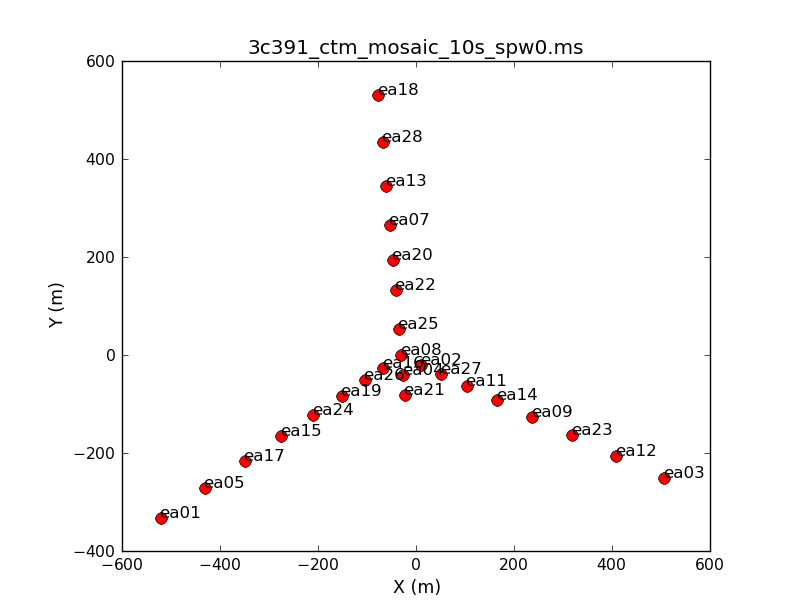
\includegraphics[scale=0.7]{../Imaging/plots/plotants_vraag12.png}
    \caption{Output of plotants() command. Here we can clearly see the antenna positions with respect to the array center. \label{fig:12b}}
\end{figure}

\noindent \textit{Question 12b) Provide the name of the centre antenna} \\
Well, either ea08 or ea21 is the name of the centre antenna. The antenna named ea08 is inside the y-shape and seems to be in the middle of that shape. The antenna ea21 is located somewhat lower and could very well be in the middle of the array as well. The log file states that ea08 is in the north array and is referred to as N01; ea08 is referred to as E01, so it is perhaps part of the East arm. Finally, if we look at W01, we see that the antenna is named ea04. All three could be in the center, but from now on I will assume ea21 is the centre antenna. \\


\noindent \textit{Question 14. 1) Amp vs. time, 2) Phase vs. time, 3) Frequency vs. time, 4) Amplitude vs. UVdist, 5)Amplitude vs. UVdist setting the item `field' in the header `data' to a value of 3, 6) Amplitude vs. UVwave.}
\begin{enumerate}
    \item See Figure~\ref{fig:14-1}.
    \item See Figure~\ref{fig:14-2}.
    \item See Figure~\ref{fig:14-3}.
    \item See Figure~\ref{fig:14-4}.
    \item See Figure~\ref{fig:14-5}.
    \item See Figure~\ref{fig:14-6}.
\end{enumerate}

\newpage

\begin{figure}[h!]
    \floatplacement{figure}{H}
    \centering
    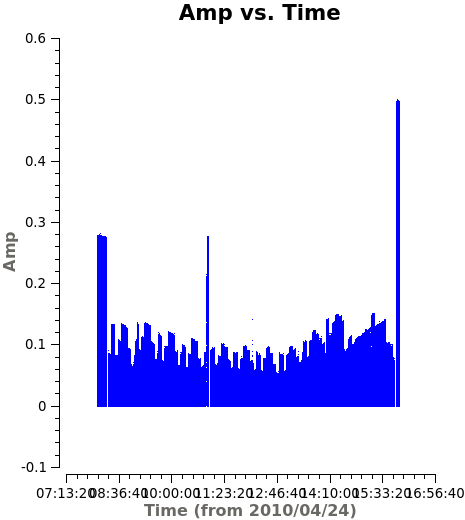
\includegraphics[scale=0.65]{../Imaging/plots/amp_vs_time_vraag14-1.png}
    \caption{Export of plotms() for Amp vs. time \label{fig:14-1}}
\end{figure}

\begin{figure}[h!]
    \floatplacement{figure}{H}
    \centering
    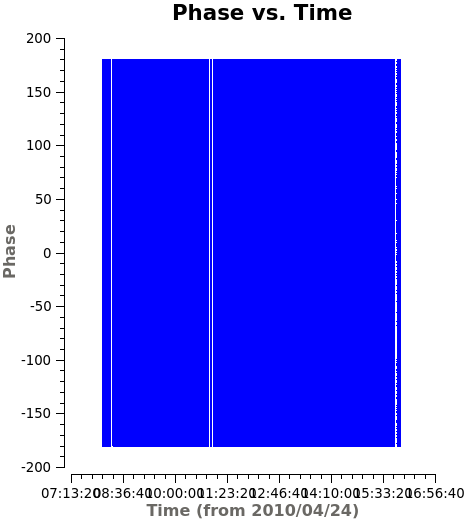
\includegraphics[scale=0.65]{../Imaging/plots/phase_vs_time_vraag14-2.png}
    \caption{Export of plotms() for Phase vs. time \label{fig:14-2}}
\end{figure}


\begin{figure}[h!]
    \floatplacement{figure}{H}
    \centering
    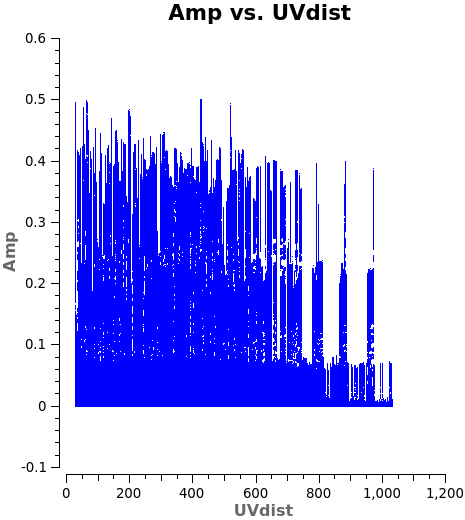
\includegraphics[scale=0.65]{../Imaging/plots/frequency_vs_time_vraag14-3.png}
    \caption{Export of plotms() for Frequency vs. time \label{fig:14-3}}
\end{figure}


\begin{figure}[h!]
    \floatplacement{figure}{H}
    \centering
    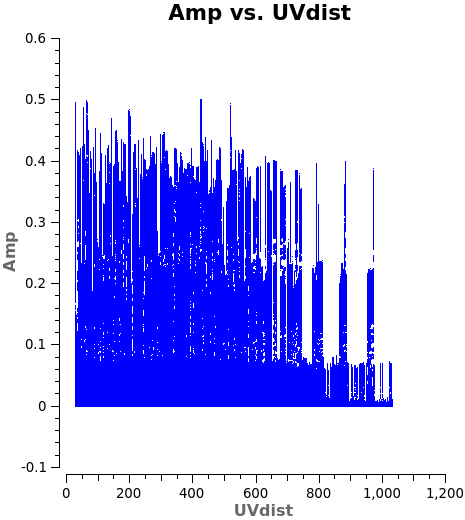
\includegraphics[scale=0.65]{../Imaging/plots/Ampltide_vs_UVdist_vraag14-4.png}
    \caption{Export of plotms() for Aplitude vs. UVdist \label{fig:14-4}}
\end{figure}


\begin{figure}[h!]
    \floatplacement{figure}{H}
    \centering
    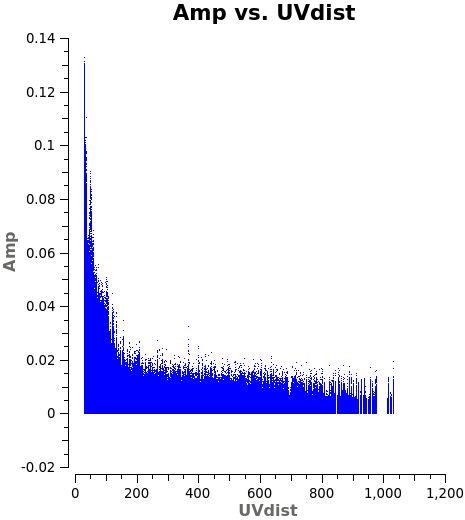
\includegraphics[scale=0.65]{../Imaging/plots/Ampltide_vs_UVdist_data-field-3_vraag14-5.png}
    \caption{Export of plotms() for Amplitude vs. UVdist setting the item `field' in the header `data' to a value of 3 \label{fig:14-5}}
\end{figure}

\begin{figure}[h!]
    \floatplacement{figure}{H}
    \centering
    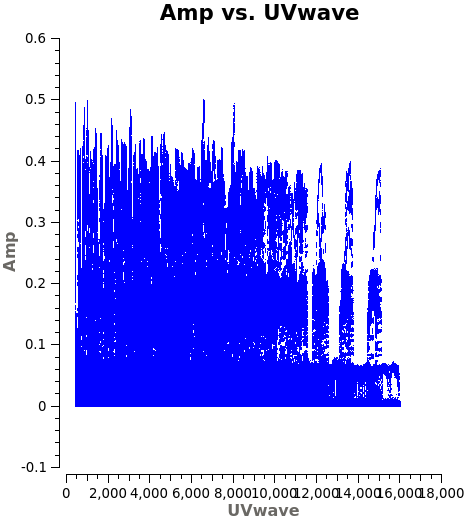
\includegraphics[scale=0.65]{../Imaging/plots/Ampltide_vs_UVwave_vraag14-6.png}
    \caption{Export of plotms() for Amplitude vs. UVwave \label{fig:14-6}}
\end{figure}

\newpage

\noindent \textit{Question 15) Submit, Amp. vs. time plot plotted above with color coded visibilities plot as shown in lecture} \\
See Figure~\ref{fig:15}. \\

\begin{figure}
    \floatplacement{figure}{H}
    \centering
    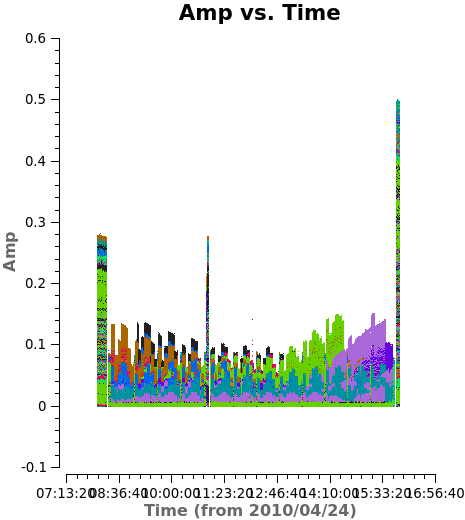
\includegraphics[scale=0.65]{../Imaging/plots/amp_vs_time_vraag15.png}
    \caption{Export of plotms() for Amp vs. time plotted with color coded visibilities as shown in lecture \label{fig:15}}
\end{figure}

\noindent \textit{Question 16) Give resolution for EVLA} \\
From the plot in question 10 we can see the outermost station names are ea18, ea01, and ea03. So we can then obtain the baselines between ea18 - ea01, ea01 - ea03, ea03 - ea18 by looking at the East and North positions from the logfile saved in question 10 (the output of the \emph{listobs()} command). By using Pythagoras theorem we can obtain three baseline values: 1031.18, 971.11, and 967.096. Now we can see that the largest baseline B is 1031.8.

From the lecture 6 slide 6 we obtain the equation $\theta = \frac{\lambda}{B}$. Again from the logfile from question 10 (the output of the \emph{listobs()} command), we obtain Ch0 (MHz), the starting frequency of the dataset $\lambda = 4536.000$ MHz. The channel width ChanWid (kHz) is $2000.000$, so the central frequency of the channel is Ch0 + ChanWid/2.

We obtain $\lambda = \frac{c}{(1031.18 \text{ m}\cdot(4536 \text{ MHz} + 1000 \text{ kHz}))} = 6.4 \cdot 10^{-5}$ radians, or $13.227$ arc seconds. \\

\noindent \textit{Question 17) Reason for difference in images 4 and 5 from question 14?} \\
Plot 5 only uses field in the header `data' set equal to 3. This means that only a single sky field is shown (number 3), which is one of the parts of the mosaic. This is in contrast to plot 4, where all sources are shown, including the calibration sources. \\

\noindent \textit{Question 18) What do you think is plot number 6 plotting?} \\
For this we take a look at the \href{http://casa.nrao.edu/Doc/Cookbook/casa_cookbook.pdf}{CASA User Reference \& Cookbook}. According to the cookbook: ``UVwave -- Projected baseline separations in units of the observing wavelength (lambda, not kilolambda). UVDist\_L is a function of frequency, and therefore, there will be a different data point for each frequency channel.'' \\

\noindent \textit{Question 19) Plot signal measured by the first antenna of each baseline} \\
Here, in the Amp vs. Antenna1 plot (Figure~\ref{fig:19-ant1}), it looks as if number 10 is not working because the amplitude seems to be like $0.02$ in contrast to the other antennas that have an amplitude of roughly $0.5$. Figure~\ref{fig:19-baseline} shows the Amp. vs. Baseline. \\

\begin{figure}
    \centering
    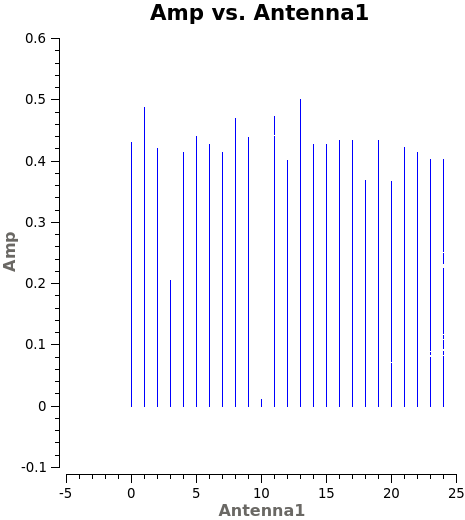
\includegraphics[scale=0.7]{../Imaging/plots/amp_vs_antenna1_vraag19.png}
    \caption{Plot of the signal measured by the first antenna of each baseline. Here we see that the fourth and eleventh line (from the left) are at roughly half the average amplitude, respectively, almost at zero. We therefore flag these antennas. \label{fig:19-ant1}}
\end{figure}

\begin{figure}
    \centering
    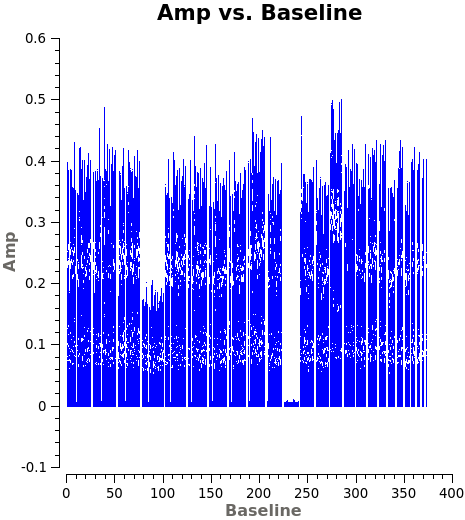
\includegraphics[scale=0.7]{../Imaging/plots/amp_vs_baseline_vraag19.png}
    \caption{Plot of the signal measured by the first antenna of each baseline: amp vs. baseline. \label{fig:19-baseline}}
\end{figure}


\section{Part2 - Flagging}
\noindent \textit{Question 1-5) The command used in CASA} \\
Here we see that the fourth and eleventh line (from the left) are at roughly half the average amplitude, respectively, almost at zero. We therefore flag these antennas. The fourth and eleventh antenna plotted in amp\_vs\_antenna1 (Figure~\ref{ig:19-ant1}) correspond to ea04, respectively, ea13, so we flag it (fourth and fifth command in the list). \\
\begin{itemize}
    \item flagdata(vis = `3c391\_ctm\_mosaic\_10s\_spw0.ms', scan=`1')
    \item flagdata(vis = `3c391\_ctm\_mosaic\_10s\_spw0.ms', mode=`quack', quackmode=`beg', quackinterval=10.0, quackincrement=False)
    \item flagdata(vis = `3c391\_ctm\_mosaic\_10s\_spw0.ms', antenna=`ea15')
    \item flagdata(vis = `3c391\_ctm\_mosaic\_10s\_spw0.ms', antenna=`ea13')
    \item flagdata(vis = `3c391\_ctm\_mosaic\_10s\_spw0.ms', antenna=`ea04')
\end{itemize}

\noindent \textit{Question 6) At the end of the flagging operation, plot the amplitude detected from each antenna.}  \\
See Figure~\ref{fig:part2-q6} for the post-flagging plot of teh amplitude detected from each antenna.
\begin{figure}
    \centering
    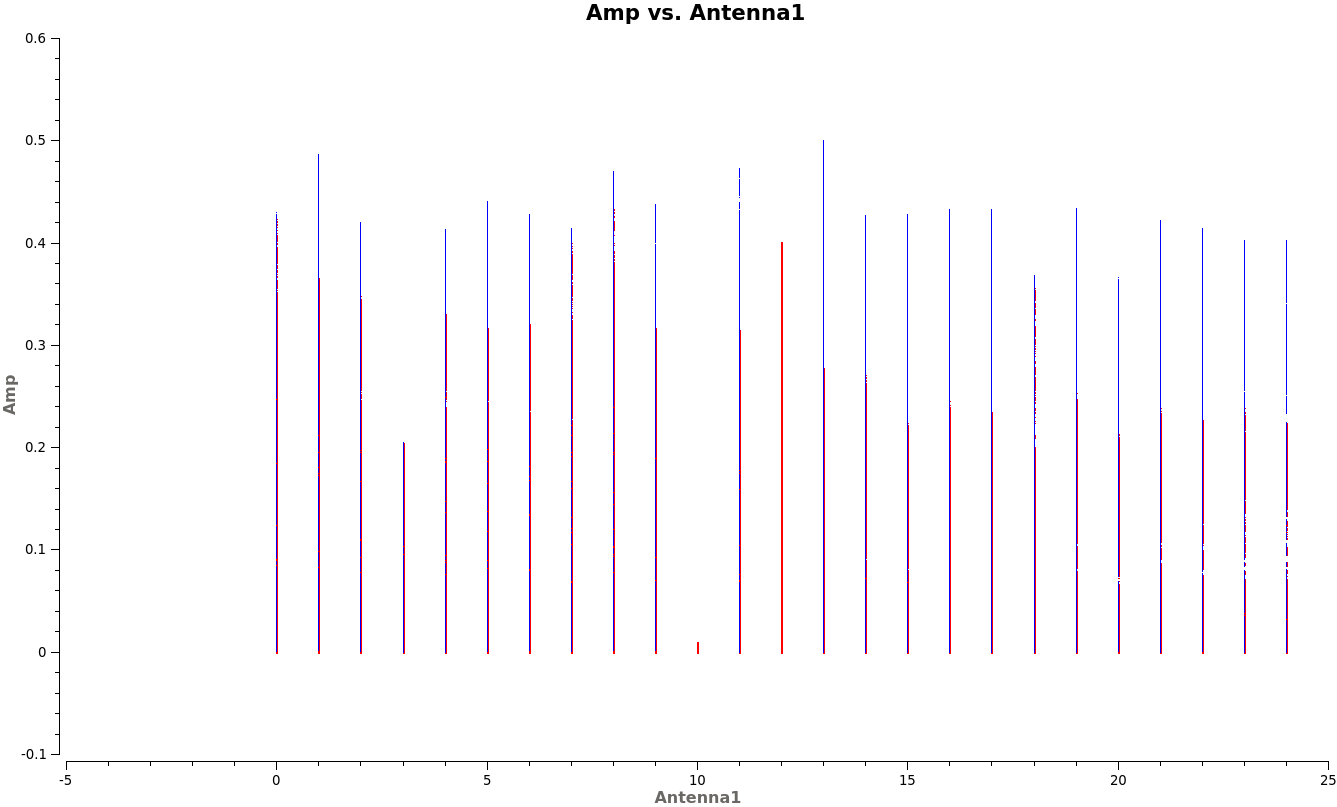
\includegraphics[scale=0.3]{../Imaging/plots/amp_vs_antenna1_part2_vraag6_with_display-FlaggedPointsSymbol-custom.png}
    \caption{Plot of the signal measure by the first antenna of each baseline post-flagging. The red color indicates flagged antennas. \label{fig:part2-q6}}
\end{figure}

\noindent \textit{Question 7) Compare the plot from above question to the amplitude vs. time plot obtained before flagging. What difference do you see?} \\
The antennas ea04 (4th from left, on x-axis at 3), ea13 (11th from left, on x-axis at 10) and ea15 (13th from left, on x-axis at 12) is now marked red. Furthermore, the full amplitude we already had is plotted blue. But now in purple a lower amplitude is reached. This might be due to the flagging of the first ten seconds required for the antenna to stabilize (the quack-mode-flagging). \\

\newpage

\section{Part 3 - Imaging}
clean(vis = `3c391\_ctm\_mosaic\_10s\_spw0.ms', imagename = `MeLoveSomeMosaicPleaseMakeThisForMeDearCasa', field=`', spw=`', mode=`mfs', niter=5000, gain=0.1, threshold=`1.0mJy', psfmode=`clark', imagermode=`mosaic', ftmachine=`mosaic', multiscale= \lbrack 0\rbrack, interactive=True, imsize=\lbrack 480, 480\rbrack, cell= \lbrack `2.5arcsec', `2.5arcsec'\rbrack, stokes=`I', weighting=`briggs', robust=0.5, usescratch=False) \\

\noindent See Figure~\ref{fig:part3} for the generated image after running the \emph{clean()} method.

\begin{figure}
    \centering
    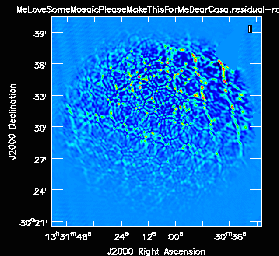
\includegraphics[scale=0.7]{../Imaging/plots/MosaicImagedPart3.png}
    \caption{Initial image post-flagging but pre-calibration. We do not yet observe something distinguishable. There are a bit more red dots in the upper left corner though. \label{fig:part3}}
\end{figure}

\section{Part 4 - Calibration}
\subsection{a. Antenna Position}
\noindent \textit{Question 1) State why and how do you think errors in antenna position can introduce an error in imaging? If the change in each position ($\Delta x_i = 0.1$ m , $\Delta y_i = 0.1$ m ) , give new sky brightness image for the Westerbork Telescope simulation . Compare this image with earlier. } \\
Well, my code requires some rewriting to implement this question. I cannot really be bothered to do so at this point in time. But if I were to change the station positions by plus or minus 0.1 meter, the number of redundant baselines will decrease and the total number of slightly different baselines will increase. This will result in a somewhat different uv-coverage. Some telescope artefacts are expected to be slightly smeared out, so to say. \\

\noindent \textit{Question 2) } \\
gencal(vis=`3c391\_ctm\_mosaic\_10s\_spw0.ms', caltable=`3c391\_ctm\_mosaic\_10s\_spw0.antpos', caltype=`antpos', spw=`', antenna=`', pol=`', parameter=\lbrack \rbrack) \\

\noindent \textit{Question 3) One line summary for what each of the options given in command in question 2} \\
The vis is the input file we are calibrating. The name of the calibration table (caltable) is specified trough the parameter `caltable'. The `spw' is the spectral window selection for specified parameters, where all spectral windows are used if left to its default. The `antenna' argument selects which antenna should be used, again leaving it empty means all antennas will be used (apart from the flagged ones obviously). The `pol' specifies which polarization will be used, where the default is all polarizations. The parameters list gives the calibration parameters to be stored in the calibration table. \\

% caltable = The new/existing calibration table
% caltype='antpos'
%     For antenna position corrections (caltype=’antpos’), the antenna  
%     position offsets are specified in the ITRF frame. For EVLA, automated  
%     lookup of the antenna position corrections is enabled when antenna is  
%     unspecified (antenna=’’) for this caltype. Note that this requires  
%     internet connection to access the EVLA antenna position correction  
%     site.  
%     For VLA position corrections in the VLA-centric frame, use  
%     caltype=’antposvla’, and gencal will rotate them to ITRF before  
%     storing them in the output caltable.  
% spw=''
%     Spectral window selection for specified parameters.  
%     default: spw=’’ (specified parameters apply to all spws)  
% antenna=''
%     Antenna selection for specified parameters.  
%     default: antenna=’’ (specified parameters apply to all antennas)  
% pol=''
%     Polarization selection for specified parameters.  
%     default: pol=’’ (specified parameters apply to all polarizations)  
% parameter=[]
%     The calibration parameters, specified as a list, to  
%     store in the caltable for the spw, antenna, and pol  
%     selection.  The required length of the list is  
%     determined by the caltype and the spw, antenna, pol  
%     selection.  One "set" of parameters (e.g., one value  
%     for ’amp’, ’ph’, etc., three values for ’antpos’)  
%     specified the same value for all indicated spw, antenna,  
%     and pol.  
%     OR,  
%     When specifying a long list of calibration parameter values,  
%     these should be ordered first (fastest) by pol (if pol!=’’),  
%     then by antenna (if antenna!=’’), and finally (sloweset) by  
%     spw (if spw!=’’).  Unspecified selection axes must not be  
%     enumerated in the parameter list  


\noindent \textit{Question 4) find out a) what different fields stand for? b) minimal and maximam values for offsets?} \\
In the logfile we see the following: 

{\tiny \noindent 2015-05-11 13:59:48	INFO	gencal::::casa	 Determine antenna position offests from the baseline correction database \\
2015-05-11 13:59:51	INFO	gencal::::casa	offsets for antenna ea01 :  0.00000   0.00300   0.00000 \\
2015-05-11 13:59:51	INFO	gencal::::casa	offsets for antenna ea02 : -0.00080   0.00000   0.00000 \\
2015-05-11 13:59:51	INFO	gencal::::casa	offsets for antenna ea03 : -0.00280   0.00000   0.00000 \\
2015-05-11 13:59:51	INFO	gencal::::casa	offsets for antenna ea05 :  0.00000   0.00280   0.00000 \\
2015-05-11 13:59:51	INFO	gencal::::casa	offsets for antenna ea11 :  0.00090   0.00000   0.00000 \\
2015-05-11 13:59:51	INFO	gencal::::casa	offsets for antenna ea12 : -0.01000   0.00450  -0.00170 \\
2015-05-11 13:59:51	INFO	gencal::::casa	offsets for antenna ea13 :  0.00000  -0.00080   0.00000 \\
2015-05-11 13:59:51	INFO	gencal::::casa	offsets for antenna ea17 : -0.00120   0.00000   0.00000 \\
2015-05-11 13:59:51	INFO	gencal::::casa	offsets for antenna ea18 :  0.00040  -0.00080   0.00040 \\
2015-05-11 13:59:51	INFO	gencal::::casa	offsets for antenna ea22 : -0.02570   0.00270  -0.01900 \\
2015-05-11 13:59:51	INFO	gencal::::casa	offsets for antenna ea23 : -0.00140   0.00000   0.00000 \\
2015-05-11 13:59:51	INFO	gencal::::casa	offsets for antenna ea24 : -0.00150   0.00000   0.00000 \\
2015-05-11 13:59:51	INFO	gencal::::casa	offsets for antenna ea26 : -0.00190   0.00000   0.00210 \\
2015-05-11 13:59:51	INFO	gencal::::casa	offsets for antenna ea27 :  0.00000   0.00190  -0.00160 } \\

From the documentation we obtain: \\
``Antenna position corrections (in the traditional VLA-centric frame) will be introduced in meters for antenna ea09 (dBx=0.01, dBy=0.02, dBz=0.03) and for antenna ea10 (dBx=-0.03, dBy=-0.01, dBz=-0.02). These offsets will be rotated to the ITRF frame before storing... ''. \\

So, the three fields are, respectively, dBx, dBy, dBz. The minimal value is 0.000000. The maximum dBx = -0.02570, dBy = 0.00450, dBz = -0.01900. These values are in meters. ITRF stands for International Terrestrial Reference Frame.

\subsection{b. Flux Density calibration}
\noindent \textit{Question 2) Refer to the listobs output in the last part 1, and here figure out the model that is used by comparing with the setjy outputs in the last step} \\ 
CASA <19>: setjy(vis=`3c391\_ctm\_mosaic\_10s\_spw0.ms', listmodels=T) \\

{\tiny \noindent Candidate modimages (*) in /opt/cep/Casa/casapy-42.1.29047-001-1-64b/data/nrao/VLA/CalModels: \\
3C138\_A.im  3C138\_L.im	3C138\_U.im  3C147\_C.im	3C147\_Q.im  3C147\_X.im	3C286\_K.im  3C286\_S.im	3C48\_A.im  3C48\_L.im  3C48\_U.im \\
3C138\_C.im  3C138\_Q.im	3C138\_X.im  3C147\_K.im	3C147\_S.im  3C286\_A.im	3C286\_L.im  3C286\_U.im	3C48\_C.im  3C48\_Q.im  3C48\_X.im \\
3C138\_K.im  3C138\_S.im	3C147\_A.im  3C147\_L.im	3C147\_U.im  3C286\_C.im	3C286\_Q.im  3C286\_X.im	3C48\_K.im  3C48\_S.im  README \\
storing them in the caltable.}  \\

In the \emph{listobs()} output we see three calibration objects identified by their field names. We have Googled these and found that J1331+3030 \href{http://casaguides.nrao.edu/index.php?title=EVLA_Continuum_Tutorial_3C391}{corresponds to} 3C286. This is the only 3C-name for which we have a model in the \emph{setjy()} output, so here I will assume this is the model to be used. The model name consists of the source name dash a letter that corresponds to the frequency band. According to Wikipedia, the IEEE system our observed frequency of 4536.000 MHz corresponds to the C band. It is concluded that we should use the model `3C286\_C.im' \\

\noindent \textit{Question 3) Report the amplitude calibrator that was used.} \\
The amplitude calibrator is \textbf{J1331+3030}. The field ID (from \emph{listobs()}). \\

\noindent \textit{Question 5a) flux density for channel 0 for every Stoke’s parameter?} \\
Here, we run setjy(vis=`3c391\_ctm\_mosaic\_10s\_spw0.ms', field=`J1331+3030', standard=`Perley-Butler 2010', model=`3C286\_C.im', usescratch=False, scalebychan=True, spw=`')

\noindent The output is: \\
{ \tiny \noindent
\{'0': \{'0': \{'fluxd': array(\lbrack 7.68301298,  0.        ,  0.        ,  0.        \rbrack)\},
       'fieldName': 'J1331+3030'\},
'format': "\{field Id: \{spw Id: \{fluxd: \lbrack I,Q,U,V\rbrack in Jy\}, 'fieldName':field name \}\}"\} 
}

\noindent From this we conclude the following
\begin{itemize}
    \item Stokes Parameter I: 7.68301298 Jy
    \item Stokes Parameter Q: 0. Jy
    \item Stokes Parameter U: 0. Jy
    \item Stokes Parameter V: 0. Jy
\end{itemize}

\noindent \textit{Question 5b) Which spectral window is used? maximum and minimum flux density scale ?} \\
{\tiny \noindent 2015-05-11 15:05:13     INFO    imager::setjy() Scaling spw 0's model image by channel to I = \lbrack 7.81908, 7.81688, 7.81468, 7.81248, 7.81028, 7.80808, 7.80588, 7.80369, 7.80149, 7.7993, 7.79711, 7.79492, 7.79273, 7.79055, 7.78836, 7.78618, 7.784, 7.78182, 7.77964, 7.77746, 7.77528, 7.77311, 7.77093, 7.76876, 7.76659, 7.76442, 7.76225, 7.76009, 7.75792, 7.75576, 7.7536, 7.75143, 7.74927, 7.74712, 7.74496, 7.7428, 7.74065, 7.7385, 7.73635, 7.7342, 7.73205, 7.7299, 7.72776, 7.72561, 7.72347, 7.72133, 7.71919, 7.71705, 7.71491, 7.71277, 7.71064, 7.70851, 7.70637, 7.70424, 7.70211, 7.69999, 7.69786, 7.69574, 7.69361, 7.69149, 7.68937, 7.68725, 7.68513, 7.68301\rbrack Jy (ch 0) for visibility prediction. } \\

So, the spectral window used is 0. The maximum is 7.81908 and the minimum 7.68301, which can be seen from the list given above. I have used the min and max function after declaring the list in Python.\\

\noindent \textit{Question 5c) Find the phase offset of image w.r.t amplitude calibrator.} \\
The model image's reference pixel is 0.00302169 arcsec from J1331+3030's phase center. \\


\subsection{c. Phase Calibration}
\noindent \textit{Question 1) List what conditions for a good phase calibrator source.} \\
From \href{https://science.nrao.edu/facilities/vla/docs/manuals/cal/referencemanual-all-pages}{The VLA Calibrator Manual} we obtain that a good phase calibrator source should: 
\begin{itemize}
    \item be in close vicinity of the source, preferably within 10 deg of the source;
    \item be one calibrator per source over the entire run;
    \item have a P or S quality status for the desired configuration and frequency;
    \item preferably be resolved, but unresolved sources could be used albeit with some caveats.
\end{itemize}

\noindent \textit{Question 2) One line summary for what each of the options given in command in question 2} \\
We run {\tiny gaincal(vis=`3c391\_ctm\_mosaic\_10s\_spw0.ms',caltable=`3c391\_ctm\_mosaic\_10s\_spw0.G0all', field=`0, 1, 9', refant=`ea21', spw=`0:27~36',  gaintype=`G', calmode=`p', solint=`int', minsnr=5, gaintable=\lbrack `3c391\_ctm\_mosaic\_10s\_spw0.antpos'\rbrack) } \\
The `vis' is the input file. The `caltable' is the calibration table used, here G0all. The `field' specifies which fields are used as calibrator fields: we know this to be 0, 1 and 9 from the \emph{listobs()} output in the log file. `refant' specifies an antenna, preferably in the center of the array (which we looked up earlier, in part 1 question 12b), with respect to which the other antennas will be calibrated. `spw' is the spectral window, `gaintype' is the type of gain solution, here `G' which means that gains are determined for each polarization and sp\_wid. The `calmode' specifies the type of solution, here `p' or phase. `solint' gives the solution interval, here `int' or per integration. `minsnr' ensures solutions with a SNR below 5 are rejected. `gaintable' again specifies the gain table calibrations to apply. \\

\noindent \textit{Question 3) What is the flagging SNR.} \\
We give minsnr=5 as input for the gaincal method. This will be the flagging SNR. \\

\noindent \textit{Question 4) Plot the gain phases in R polarization for at least 4 antennae.} \\
We run {\tiny plotcal(caltable=`3c391\_ctm\_mosaic\_10s\_spw0.G0all',xaxis=`time',yaxis=`phase', poln=`R',iteration=`antenna',plotrange=\lbrack -1,-1,-180,180\rbrack) }  \\
See Figure~\ref{fig:part4subC2-1} for the gain phase plot of the first antenna, Figure~\ref{fig:part4subC2-2} for the reference antenna `ea21', Figure~\ref{fig:part4subC2-3} for the plot of `ea05' (which we flagged due to the fluctuations), and Figure~\ref{fig:part4subC2-4} for the plot of an antenna (`ea24') with interesting behaviour. We did not flag the latter, because the gain phase does follow a straight line albeit a non-horizontal but an increasing line as a function of time. 

\newpage 

\begin{figure}[h!]
    \floatplacement{figure}{H}
    \centering
    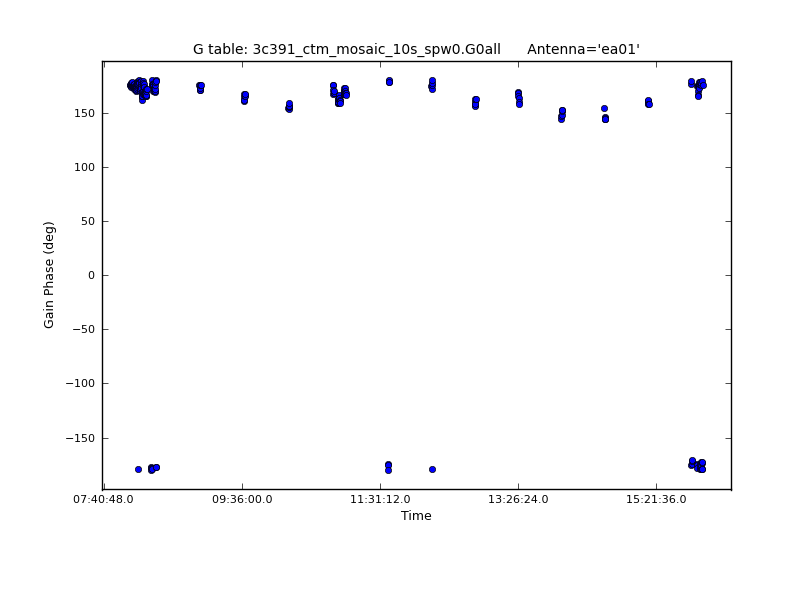
\includegraphics[scale=0.5]{../Imaging/plots/phase_calibration_part4c_question5_ea01.png}
    \caption{Output of \emph{plotcal()} for antenna `ea01', the first antenna. \label{fig:part4subC2-1}}
\end{figure}

\begin{figure}[h!]
    \floatplacement{figure}{H}
    \centering
    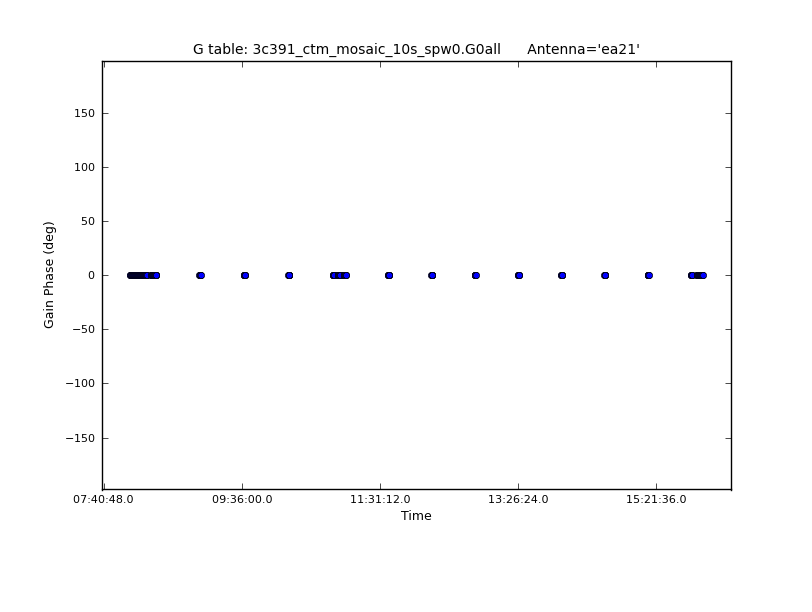
\includegraphics[scale=0.5]{../Imaging/plots/phase_calibration_part4c_question5_ea21.png}
    \caption{Output of \emph{plotcal()} for antenna `ea21', the reference antenna. \label{fig:part4subC2-2}}
\end{figure}

\begin{figure}[h!]
    \floatplacement{figure}{H}
    \centering
    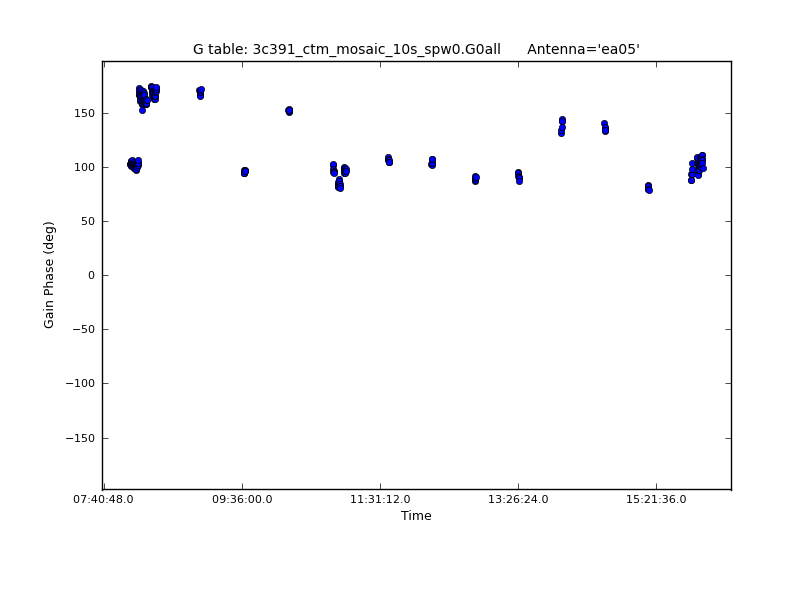
\includegraphics[scale=0.5]{../Imaging/plots/phase_calibration_part4c_question5_ea05.png}
    \caption{Output of \emph{plotcal()} for antenna `ea05', the antenna flagged because of the fluctuations. \label{fig:part4subC2-3}}
\end{figure}

\begin{figure}[h!]
    \floatplacement{figure}{H}
    \centering
    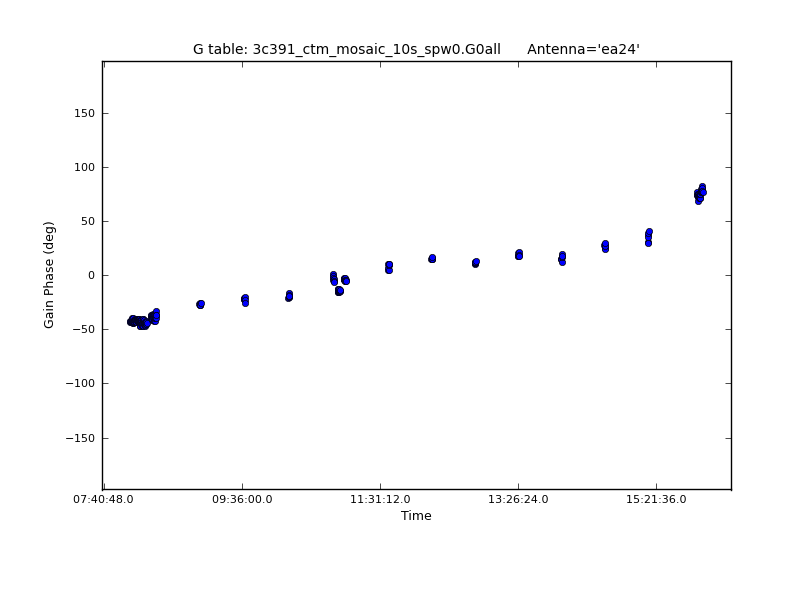
\includegraphics[scale=0.5]{../Imaging/plots/phase_calibration_part4c_question5_ea24.png}
    \caption{Output of \emph{plotcal()} for antenna `ea24'. We show this because the gain phase does have a straight line but it is increasing (not horizontal). We did not flag this antenna though. \label{fig:part4subC2-4}}
\end{figure}
\newpage


\noindent \textit{Question 5) Report antennae for which in phase gains you see sudden jumps.} \\
Antenna ea05 in R polarization has a variation of 150. The other antennas have variations of at most 50. There are some plots where it seems as if there are two populations, but they lie at roughly the same value with either a plus or a minus sign. I think this might be oke, although I have no idea if I should flag this. But if I do flag all of these antenna's, almost no data is left. After discussing this with Amruta, the plus or minus sign does not matter, so we only flag ea05 because it looks strange in R polarization, and we flag ea12 because it looks strange in L polarization. \\

\noindent \textit{Question 6) } \\
\noindent Here, we run the following two commands: \\
{\tiny flagdata(vis=`3c391\_ctm\_mosaic\_10s\_spw0.ms', flagbackup=T, mode=`manual', antenna=`ea05') \\
\noindent flagdata(vis=`3c391\_ctm\_mosaic\_10s\_spw0.ms', flagbackup=T, mode=`manual', antenna=`ea12') \\ }
% 
\noindent \textit{Question 8) Plot the gain phases in L polarization for at least 4 antennae.} \\
COMMAND TO RUN ON CEP3 REPLACE REPLACE

\subsection{d. Delay Calibration}
First, we run {\tiny gaincal(vis=`3c391\_ctm\_mosaic\_10s\_spw0.ms',caltable=`3c391\_ctm\_mosaic\_10s\_spw0.K0', field=`J1331+3030',refant=`ea21',spw=`0:5~58',gaintype=`K', solint=`inf',combine=`scan',minsnr=5, gaintable=\lbrack `3c391\_ctm\_mosaic\_10s\_spw0.antpos', `3c391\_ctm\_mosaic\_10s\_spw0.G0'\rbrack)}. \\
\noindent \textit{Question 2) Plot for the time delays for each antenna.} \\
{\tiny plotcal(caltable=`3c391\_ctm\_mosaic\_10s\_spw0.K0',xaxis=`antenna',yaxis=`delay', figfile=`plotcal\_3c391-K0-delay.png') } \\
See Figure~\ref{fig:part4subD} for the plot of the delay calibration.

\begin{figure}[h!]
    \floatplacement{figure}{H}
    \centering
    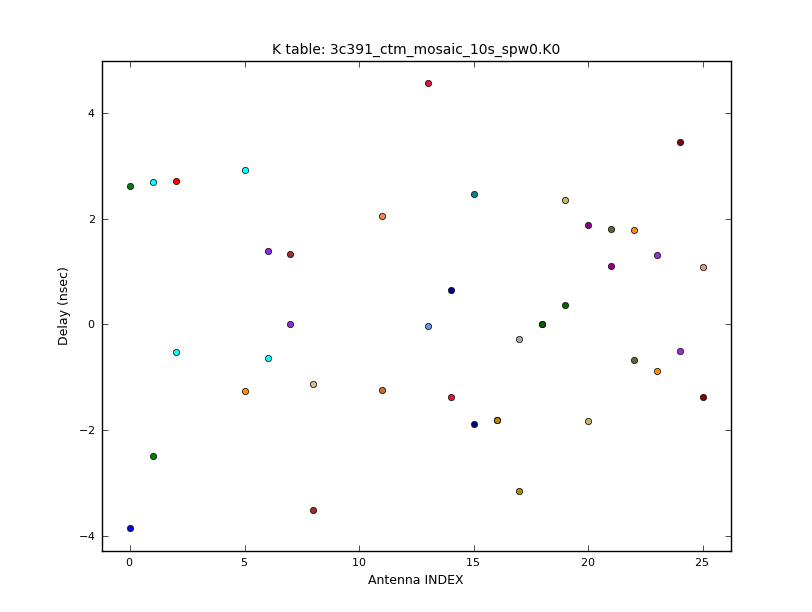
\includegraphics[scale=0.65]{../Imaging/plots/plotcal_3c391-K0-delay.png}
    \caption{Output of \emph{plotcal()} for the K0 caltable. Here we see the time delays for each antenna. \label{fig:part4subD}}
\end{figure}
 
\subsection{e. Bandpass Calibration}
\noindent \textit{Question 1) Find out if a synthesized beam size is given what will be the positional uncertainty for spectral feature?} \\
This question might be somewhat too difficult for me to answer. \\

\noindent \textit{Question 3a) Plot the gain phases in R polarization for all antennae. Now using plotcal we can plot four plots: Ampl R polarization, L polarization} \\
See Figure~\ref{fig:part4subE-q3a-R} for the R polarization, and Figure~\ref{fig:part4subE-q3a-L} for the L polarization. \\

\newpage
\begin{figure}[h!]
    \floatplacement{figure}{H}
    \centering
    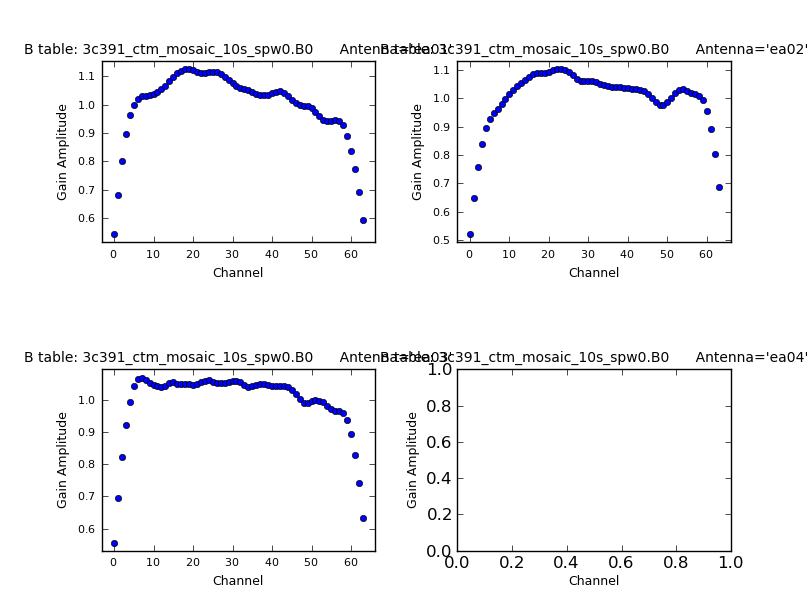
\includegraphics[scale=0.5]{../Imaging/plots/part4-subE-question3a_amp_pol-R.png}
    \caption{Output of \emph{plotcal()}  \label{fig:part4subE-q3a-R}}
\end{figure}
\begin{figure}[h!]
    \floatplacement{figure}{H}
    \centering
    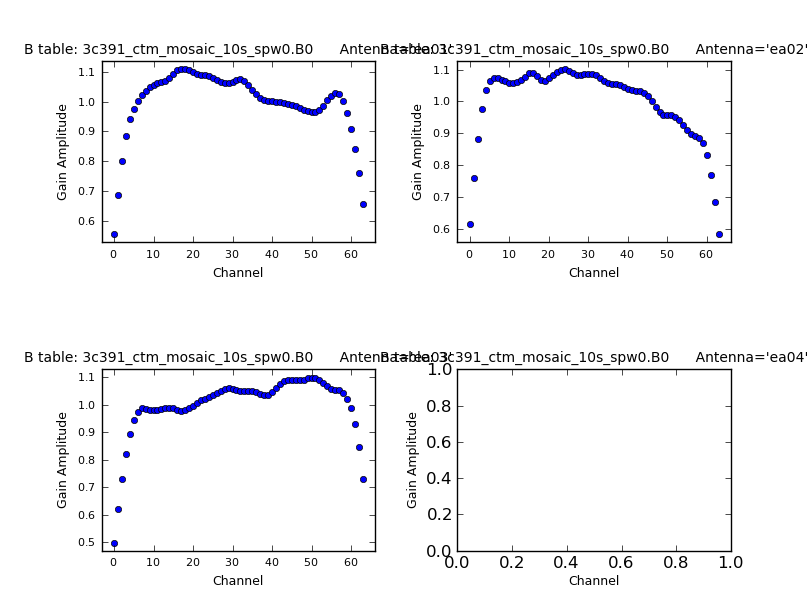
\includegraphics[scale=0.5]{../Imaging/plots/part4-subE-question3a_amp_pol-L.png}
    \caption{Output of \emph{plotcal()}  \label{fig:part4subE-q3a-L}}
\end{figure}
\newpage

\noindent \textit{Question 3b) Plot the gain phases in R polarization for all antennae. Now using plotcal we can plot four plots: Phase R polarization, L polarization} \\
See Figure~\ref{fig:part4subE-q3b-R} for the R polarization, and Figure~\ref{fig:part4subE-q3b-L} for the L polarization. \\

\newpage
\begin{figure}[h!]
    \floatplacement{figure}{H}
    \centering
    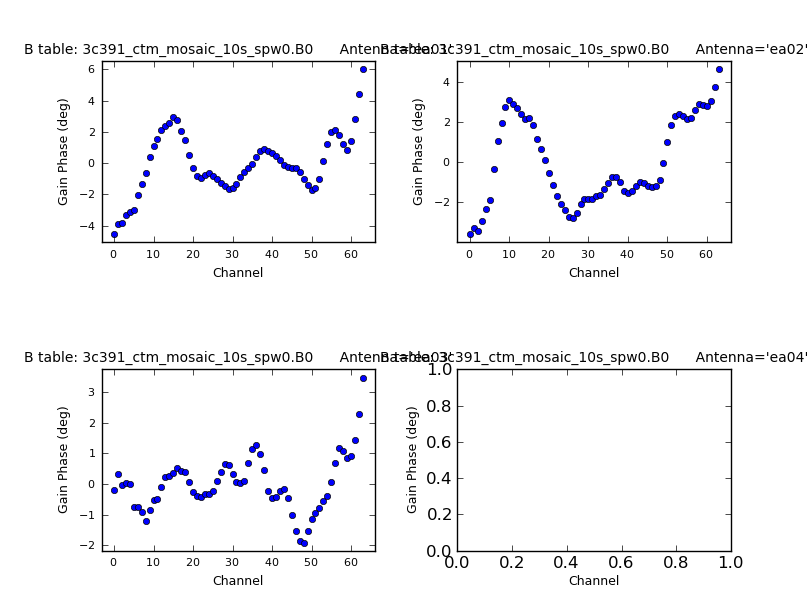
\includegraphics[scale=0.5]{../Imaging/plots/part4-subE-question3b_phase_pol-R.png}

    \caption{Output of \emph{plotcal()}  \label{fig:part4subE-q3b-R}}
\end{figure}
\begin{figure}[h!]
    \floatplacement{figure}{H}
    \centering
    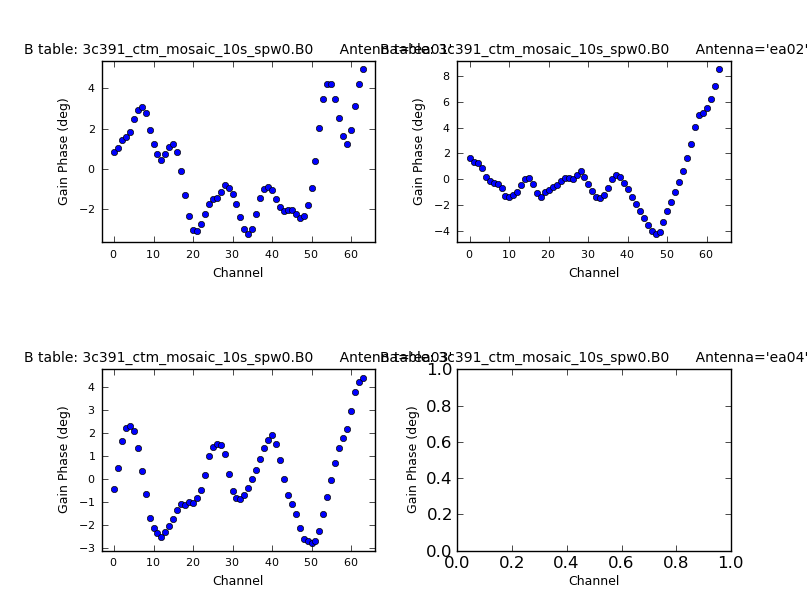
\includegraphics[scale=0.5]{../Imaging/plots/part4-subE-question3b_phase_pol-L.png}
/
    \caption{Output of \emph{plotcal()}  \label{fig:part4subE-q3b-L}}
\end{figure}
\newpage

% part4-subE-question3b_phase_pol-L.png ??
% part4-subE-question3b_phase_pol-R.png ??


\subsection{f. Gain Calibration}
\noindent \textit{Question) Report the phase calibrator being used by you.} \\
The used phase calibrator is \textbf{J1822-0938}. The polarization calibrator is \textbf{J0319+4130}, or \textbf{3C84}.\\


% 1)
% gaincal(vis='3c391\_ctm\_mosaic\_10s\_spw0.ms', caltable='3c391\_ctm\_mosaic\_10s\_spw0.G1', field='J1331+3030', spw='0:5~58', solint='inf', refant='ea21', gaintype='G', calmode='ap', solnorm=F, gaintable=['3c391\_ctm\_mosaic\_10s\_spw0.antpos', '3c391\_ctm\_mosaic\_10s\_spw0.K0', '3c391\_ctm\_mosaic\_10s\_spw0.B0'])
% 
% 2)
% gaincal(vis='3c391\_ctm\_mosaic\_10s\_spw0.ms', caltable='3c391\_ctm\_mosaic\_10s\_spw0.G1', field='J1822-0938', spw='0:5~58', solint='inf', refant='ea21', gaintype='G', calmode='ap', gaintable=['3c391\_ctm\_mosaic\_10s\_spw0.antpos', '3c391\_ctm\_mosaic\_10s\_spw0.K0', '3c391\_ctm\_mosaic\_10s\_spw0.B0'], append=True)
% 
% 3) The polarization calibration source is J0319+4130, or 3C 84.
% gaincal(vis='3c391\_ctm\_mosaic\_10s\_spw0.ms', caltable='3c391\_ctm\_mosaic\_10s\_spw0.G1', field='J0319+4130', spw='0:5~58', solint='inf', refant='ea21', gaintype='G', calmode='ap', gaintable=['3c391\_ctm\_mosaic\_10s\_spw0.antpos', '3c391\_ctm\_mosaic\_10s\_spw0.K0', '3c391\_ctm\_mosaic\_10s\_spw0.B0'], append=True)
% 
\noindent \textit{Question 4) } \\
% plotcal(caltable='3c391\_ctm\_mosaic\_10s\_spw0.G1', xaxis='time', yaxis='amp', poln='L', figfile='part4-subF-question4\_amp\_pol-L.png')
% 
% plotcal(caltable='3c391\_ctm\_mosaic\_10s\_spw0.G1', xaxis='time', yaxis='amp', poln='R', figfile='part4-subF-question4\_amp\_pol-R.png')
% 
% plotcal(caltable='3c391\_ctm\_mosaic\_10s\_spw0.G1', xaxis='time', yaxis='phase', poln='L', plotrange=[-1,-1,-180,180], figfile='part4-subF-question4\_phase\_pol-L.png')
% 
% plotcal(caltable='3c391\_ctm\_mosaic\_10s\_spw0.G1', xaxis='time', yaxis='phase', poln='R', plotrange=[-1,-1,-180,180], figfile='part4-subF-question4\_phase\_pol-R.png')
% 
% 
\noindent \textit{Question 4) Plot the phase and amplitude gain solutions for each of the L and R polarizations} \\
See Figure~\ref{fig:part4subF-amp-R} for the gain calibration amp plot for pol R, Figure~\ref{fig:part4subF-amp-L} for the amp for pol L; Figure~\ref{fig:part4subF-phase-R} for the gain calibration phase plot for pol R, and Figure~\ref{fig:part4subF-phase-L} for the phase for pol L.
\newpage
\begin{figure}[h!]
    \floatplacement{figure}{H}
    \centering
    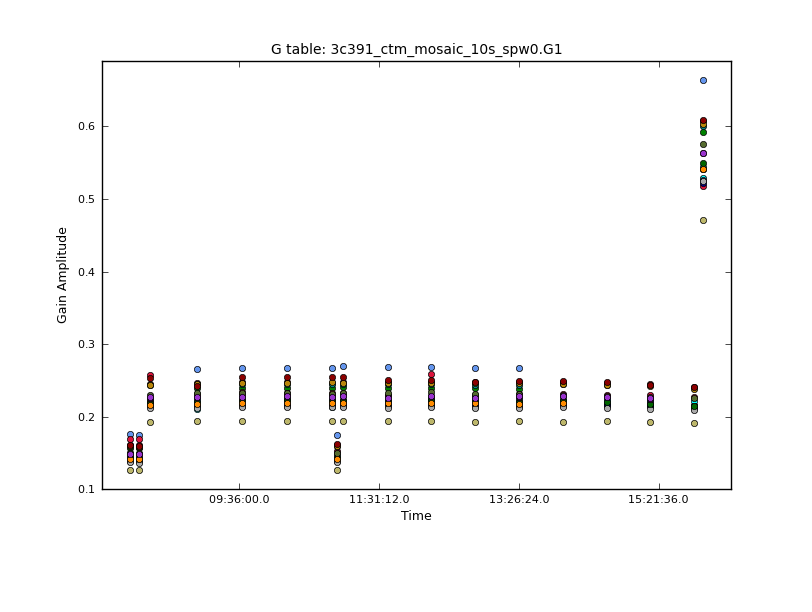
\includegraphics[scale=0.5]{../Imaging/plots/part4-subF-question4_amp_pol-R.png}

    \caption{Output of \emph{plotcal()} for the gain calibration - amp for pol R. \label{fig:part4subF-amp-R}}
\end{figure}
\begin{figure}[h!]
    \floatplacement{figure}{H}
    \centering
    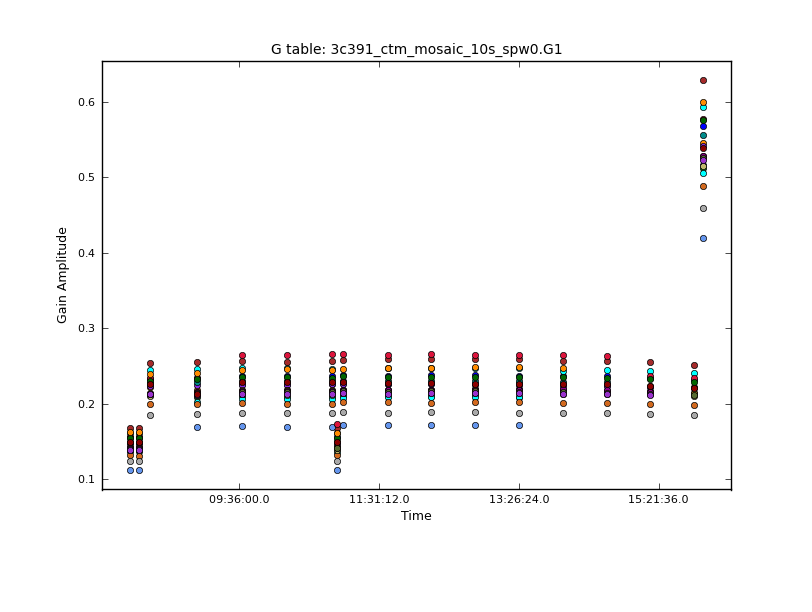
\includegraphics[scale=0.5]{../Imaging/plots/part4-subF-question4_amp_pol-L.png}
    \caption{Output of \emph{plotcal()} for the gain calibration - amp for pol L. \label{fig:part4subF-amp-L}}
\end{figure}
\newpage
\begin{figure}[h!]
    \floatplacement{figure}{H}
    \centering
    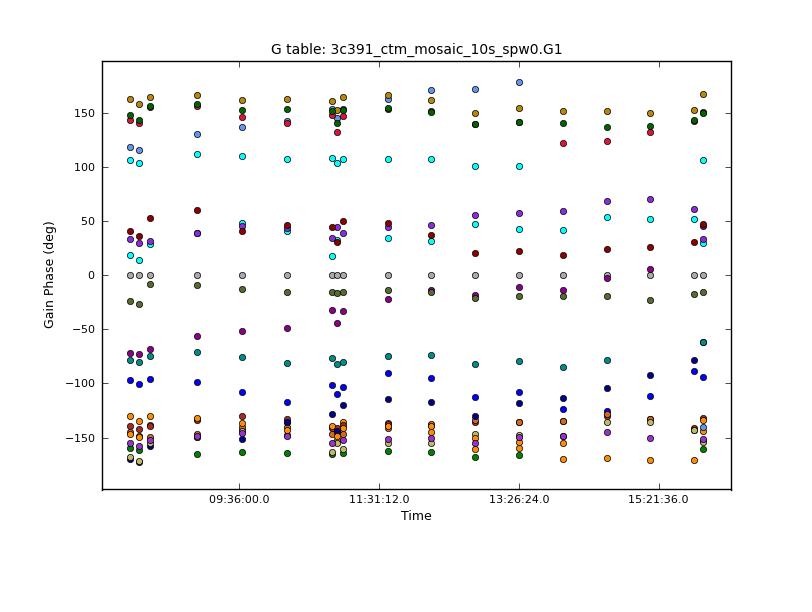
\includegraphics[scale=0.5]{../Imaging/plots/part4-subF-question4_phase_pol-R.png}
    \caption{Output of \emph{plotcal()} for the gain calibration - phase for pol R. \label{fig:part4subF-phase-R}}
\end{figure}
\begin{figure}[h!]
    \floatplacement{figure}{H}
    \centering
    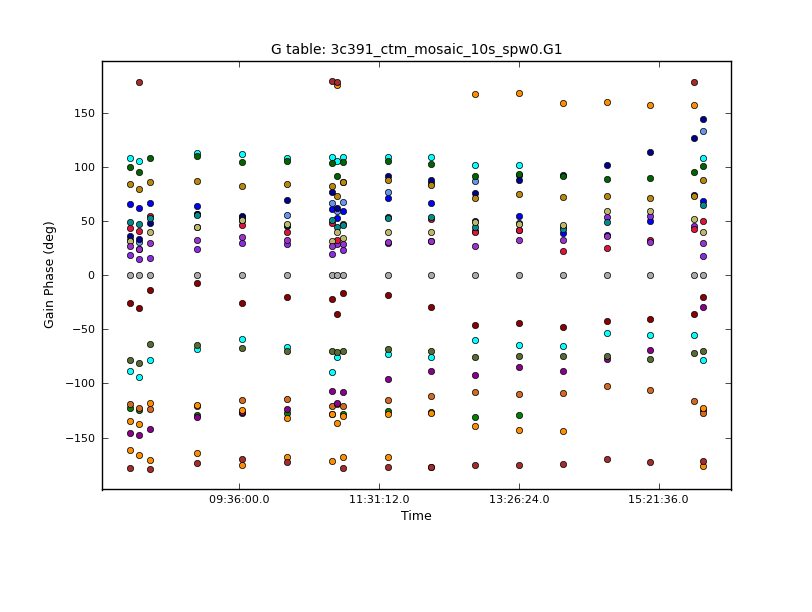
\includegraphics[scale=0.5]{../Imaging/plots/part4-subF-question4_phase_pol-L.png}
    \caption{Output of \emph{plotcal()} for the gain calibration - phase for pol L. \label{fig:part4subF-phase-L}}
\end{figure}
\newpage

\subsection{g. Scaling the amplitude gains}
The command run is {\tiny myscale = fluxscale(vis=`3c391\_ctm\_mosaic\_10s\_spw0.ms', caltable=`3c391\_ctm\_mosaic\_10s\_spw0.G1', fluxtable=`3c391\_ctm\_mosaic\_10s\_spw0.fluxscale1', reference=\lbrack`J1331+3030'\rbrack, transfer=\lbrack`J1822-0938, J0319+4130'\rbrack, incremental=False) } \\
\noindent \textit{Question 3) What flux density scale do you obtain for secondary calibrator? Signal to noise ratio (SNR) printed for given calibrator field? } \\
From the logfile we obtain (if we only keep the two relevant lines): \\

{\tiny \noindent 2015-05-11 21:49:18     INFO    fluxscale::::    Flux density for J1822-0938 in SpW=0 (freq=4.536e+09 Hz) is: 2.34094 +/- 0.00625394 (SNR = 374.314, N = 42) \\
2015-05-11 21:49:18     INFO    fluxscale::::    Flux density for J0319+4130 in SpW=0 (freq=4.536e+09 Hz) is: 13.9306 +/- 0.0331459 (SNR = 420.281, N = 42) \\ }

From this, we can easily read the SNR value. For J1822-0938 the SNR = 374.314, N=42; for J0319+4130 the SNR = 420.281, N=42. \\

\noindent \textit{Question 4) U se VLA calibrator manual and report if flux density you obtained for the secondary calibrators look fine.} \\

\noindent Using \url{http://www.vla.nrao.edu/astro/calib/manual/csource.html} we obtain \\
\noindent \textbf{for J1822-0938}: \\
{\tiny \noindent 822-096   J2000  T 18h22m28.7042s   -09d38'56.835" \\
819-096   B1950  T 18h19m43.5900s   -09d40'29.000" \\
---------------------------------------------------- \\
AND        A B C D    FLUX(Jy)    UVMIN(kL)  UVMAX(kL) \\
==================================================== \\
90cm    P  S S S S         13 \\
20cm    L  X P P P        5.6                       50 \\
.7cm    X  X X S P        1.3                       50 \\
.7cm    Q  W W W W       0.20 \\ }

Here, we use the C band. However, the C band is not represented in this table, but the X band of 3.7 cm is closest to 6 cm. So the value we find should be above 1.3 Jy but well below 5.6 Jy. The obtained value of 2.34094 Jy does not look too weird or surprising, I think. \\

\noindent \textbf{for J0319+4130 we obtain}:\\
{\tiny \noindent 319+415   J2000  B 03h19m48.160102s  41d30'42.103050"  Aug01  3C84 \\
316+413   B1950  B 03h16m29.567300s  41d19'51.916000" \\
---------------------------------------------------- \\
AND        A B C D    FLUX(Jy)    UVMIN(kL)  UVMAX(kL) \\
==================================================== \\
90cm    P  S X X X          8           13 \\
20cm    L  P P X X      23.9            12 \\
 6cm    C  P P P P      23.3 \\
.7cm    X  P P P P      21.70                       visplot \\
 2cm    U  P P P P      20.70                       visplot \\
.3cm    K  X S S S      16.4  \\
.7cm    Q  X S S S       9.00                      1800   visplot \\}

Here, we use the C band, so we expect the FLUX to be 23.3 Jy? We obtain 13.9306, however, which is like 10 lower. This slightly concerns me, although I do not know what difference should be considered worrysome. I mean, it is the same order of magnitide, right? \\

\noindent \textit{Question 5) Plot the rescaled amplitudes for R and L polarizations.} \\
See Figure~\ref{fig:part4subG-amp-R} and Figure~\ref{fig:part4subG-amp-L} for the rescaled amplitudes of the R and L polarizations.
\newpage
\begin{figure}[h!]
    \floatplacement{figure}{H}
    \centering
    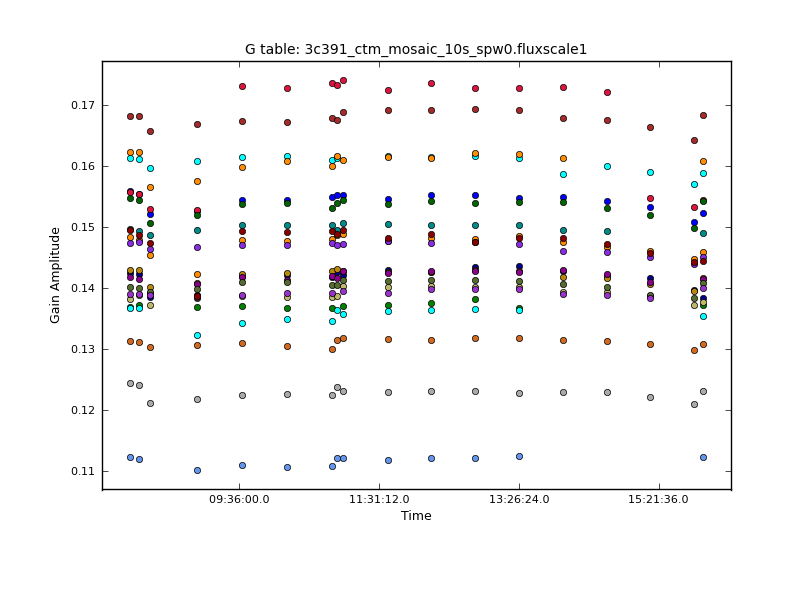
\includegraphics[scale=0.5]{../Imaging/plots/part4-subG-question5_amp_pol-L.png}
    \caption{Output of \emph{plotcal()} for the gain calibration - amp for pol R - rescaled. \label{fig:part4subG-amp-R}}
\end{figure}
\begin{figure}[h!]
    \floatplacement{figure}{H}
    \centering
    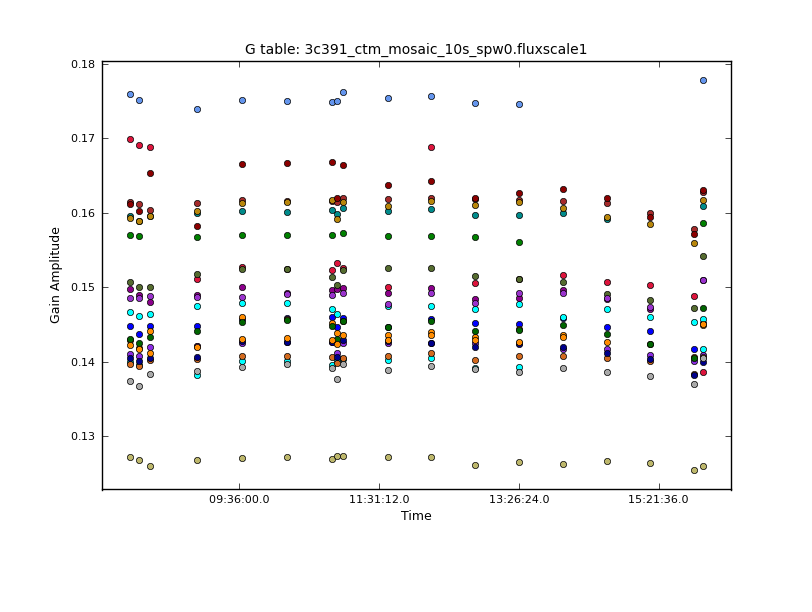
\includegraphics[scale=0.5]{../Imaging/plots/part4-subG-question5_amp_pol-R.png}
    \caption{Output of \emph{plotcal()} for the gain calibration - amp for pol L - rescaled. \label{fig:part4subG-amp-L}}
\end{figure}
\newpage





% plotcal(caltable='3c391\_ctm\_mosaic\_10s\_spw0.fluxscale1', xaxis='time', yaxis='amp', poln='R', figfile='part4-subG-question5\_amp\_pol-R.png')
% plotcal(caltable='3c391\_ctm\_mosaic\_10s\_spw0.fluxscale1', xaxis='time', yaxis='amp', poln='L', figfile='part4-subG-question5\_amp\_pol-L.png')
% 
% 

\section{Applying Calibrations}
\noindent \textit{Question 3a) Now, that the visibilities are well calibrated. Make standard plots again with plotcal: field 0 corrected phase and amplitudes. } \\
See Figure~\ref{fig:part4subH-amp-0} and Figure~\ref{fig:part4subH-phase-0} for the post-calibration plot of field 0, respectively the corrected amplitude and phase. \\
\newpage
\begin{figure}[h!]
    \floatplacement{figure}{H}
    \centering
    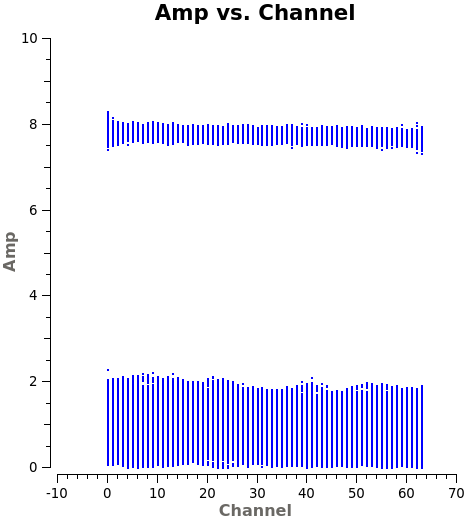
\includegraphics[scale=0.5]{../Imaging/plots/part4-subH-question3_fld0-corrected-amp.png}
    \caption{Output of \emph{plotcal()} field 0 corrected amplitude plot. \label{fig:part4subH-amp-0}}
\end{figure}
\begin{figure}[h!]
    \floatplacement{figure}{H}
    \centering
    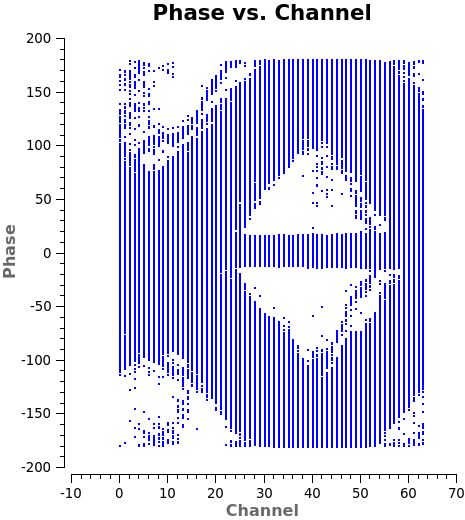
\includegraphics[scale=0.5]{../Imaging/plots/part4-subH-question3_fld0-corrected-phase.png}
    \caption{Output of \emph{plotcal()} field 0 corrected phase plot. \label{fig:part4subH-phase-0}}
\end{figure}
\newpage
\noindent \textit{Question 3b) Now, that the visibilities are well calibrated. Make standard plots again with plotcal: field 1 corrected phase and amplitudes.} \\
% See Figure~\ref{fig:part4subH-amp-1} and Figure~\ref{fig:part4subH-phase-1} for the post-calibration plot of field 1, respectively the corrected amplitude and phase. \\
% \newpage
% \begin{figure}[h!]
%     \floatplacement{figure}{H}
%     \centering
%     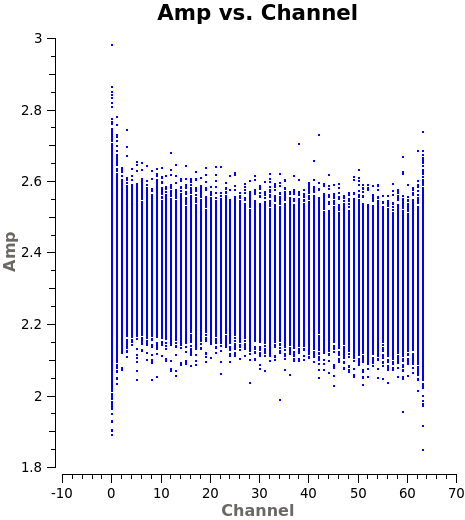
\includegraphics[scale=0.5]{../Imaging/plots/part4-subH-question3_fld1-corrected-amp.png}
%     \caption{Output of \emph{plotcal()} field 1 corrected amplitude plot. \label{fig:part4subH-amp-1}}
% \end{figure}
% \begin{figure}[h!]
%     \floatplacement{figure}{H}
%     \centering
%     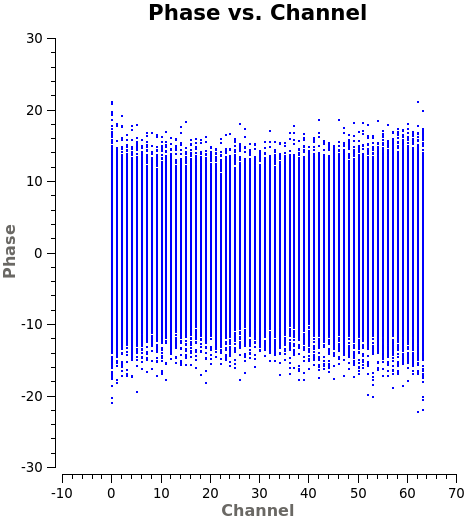
\includegraphics[scale=0.5]{../Imaging/plots/part4-subH-question3_fld1-corrected-phase.png}
%     \caption{Output of \emph{plotcal()} field 1 corrected phase plot. \label{fig:part4subH-phase-1}}
% \end{figure}
% \newpage


\noindent \textit{Question 4) Plot amplitude vs. phase, centered around zero phase for field/ amplitude calibrator.} \\
See Figure~\ref{fig:part4subH-ellips} for the plot of the amplitude vs. phase. 
\begin{figure}[h!]
    \floatplacement{figure}{H}
    \centering
    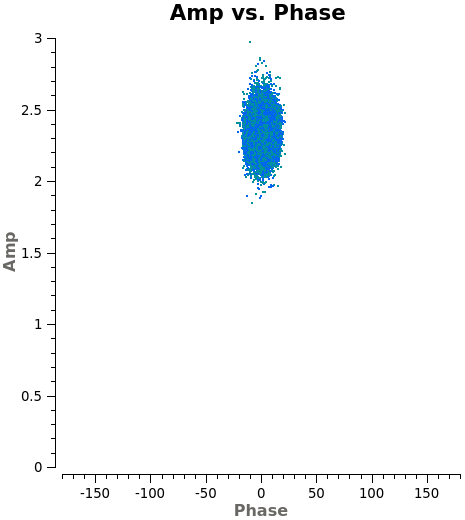
\includegraphics[scale=0.5]{../Imaging/plots/part4-subH-question4_fld1-corrected-ampvsphase.png}
    \caption{Output of \emph{plotcal()} - plot of amplitude vs. phase centered around zero phase. Here we expect to see a circle at the phase equal zero, but we notice an ellipse: close enough! \label{fig:part4subH-ellips}}
\end{figure}

\section{Part 5 - Imaging}
{\tiny clean(vis=`3c391\_ctm\_mosaic\_10s\_spw0.ms', imagename=`part5-question2\_initial', field=`', spw=`', mode=`mfs', niter=5000, gain=0.1, threshold=`1.0mJy', psfmode=`clark', imagermode=`mosaic', ftmachine=`mosaic', multiscale=\lbrack 0\rbrack, interactive=True, imsize=\lbrack 480, 480\rbrack, cell=\lbrack `2.5arcsec', `2.5arcsec'\rbrack, stokes=`I', weighting=`briggs', robust=0.5, usescratch=False) }

\noindent \textit{Question) What do you observe now compare it with pre calibration image list changes?} \\
Now we do actually see something reminiscent of a supernova remnant as opposed to the pre-calibration image, where I cannot really tell what it is that I am seeing.
\end{document}
